\documentclass[12pt,a4paper]{article}

% --- Paquetes Básicos ---
\usepackage[utf8]{inputenc}
\usepackage[T1]{fontenc}
\usepackage{graphicx} 
\usepackage{geometry} 
\usepackage{setspace} 

% --- Soporte para Español y Cambio de Nombres ---
\usepackage[spanish]{babel} % Configura el idioma español

\addto\captionsspanish{
    \renewcommand{\contentsname}{Índice general} % Cambia "Contents" a "Índice general"
    \renewcommand{\refname}{Bibliografía}        % Cambia "References" a "Bibliografía"
}

% --- Configuración de márgenes generales ---
\geometry{
	left=3cm,
	right=2.5cm,
	top=2.5cm,
	bottom=2.5cm
}

\begin{document}
	
	% ------------------- PORTADA -------------------
	\begin{titlepage}
		% Ajuste de márgenes solo para la portada
		\newgeometry{left=1.5cm, right=1.5cm, top=1.5cm, bottom=1.5cm}
		
		\noindent
		% Columna Izquierda: Imagen decorativa azul (uo-big.png)
		\begin{minipage}[c][\textheight][c]{0.35\textwidth}
			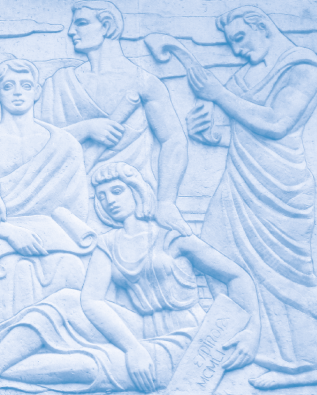
\includegraphics[width=\linewidth, height=\textheight, keepaspectratio=false]{uo-big.png}
		\end{minipage}
		\hfill
		% Columna Derecha: Información institucional y título
		\begin{minipage}[c][\textheight][t]{0.70\textwidth}
			\vspace{1cm}
			\begin{center}
				
\includegraphics[width=0.8\linewidth]{logo.png} \\[0.5cm]
				
				{\Large \textbf{UNIVERSIDAD DE ORIENTE}} \\[0.7cm]
			
				{\large \textbf{FACULTAD DE CIENCIAS NATURALES Y EXACTAS}} \\[0.8cm]
			
				{\large \textbf{DEPARTAMENTO DE CIENCIAS DE LA COMPUTACIÓN}} \\[0.8cm]

                {\large \textbf{TERCER AÑO LICENCIATURA CIENCIAS DE LA COMPUTACIÓN}} \\[0.5cm]
				
				\vfill
				
				{\Large \textbf{Información extra sobre el trabajo}} \\[0.8cm] 
				{\LARGE \bfseries Título del trabajo:} \\[2.5cm]
				
				\vfill
			\end{center}
			
			\begin{flushright}
				{\large \textbf{Autora:}} \\
				{\large Solji Charón Peña} \\[0.5cm]
				{\large \textbf{Tutora:}} \\
				{\large Nombre}
			\end{flushright}
			
			\vfill
			
			\begin{center}
				{\large \today}
			\end{center}
		\end{minipage}
		
		\restoregeometry
	\end{titlepage}
	
	% --- Configuración de interlineado ---
	\onehalfspacing % 1.5 es el estándar académico; usa \doublespacing si lo prefieres
	
	% ------------------- RESUMEN Y ABSTRACT -------------------
	\section*{Resumen}
	\addcontentsline{toc}{section}{Resumen}
		
	\vspace{0.5cm}
	\noindent\textbf{Palabras clave:} 
	
	\newpage
	
	\section*{Abstract}
	\addcontentsline{toc}{section}{Abstract}
	
	\vspace{0.5cm}
	\noindent\textbf{Keywords:} 
	
	\newpage
	
	% ------------------- ÍNDICE -------------------
	\tableofcontents
	\newpage
	
	% ------------------- CONTENIDO -------------------
	\newpage
	\section*{Introducción}
	\newpage
	\section*{Desarrollo}
	\section {Sección de ejemplo}
	
	\subsection{Subsección de ejemplo}
	\newpage
	\section*{Conclusiones}
	
	\newpage
	
	% ------------------- BIBLIOGRAFÍA -------------------
	\begin{thebibliography}{99}
		\addcontentsline{toc}{section}{Bibliografía}
		

		
		
	\end{thebibliography}
	
\end{document}